\documentclass[a4paper]{report}

\usepackage{a4wide}
% To decrease the margins and allow more text on a page.

\usepackage{graphicx}
% To deal with including pictures.

\usepackage{enumerate}
% To provide a little bit more functionality than with LaTeX's default
% enumerate environment.

\usepackage{array}
% To provide a little bit more functionality than with LaTeX's default
% array environment.

\usepackage[parfill]{parskip}

\usepackage{multicol}
% For if we want to put something in a multi column environment.

\usepackage{float}
% For if we want to put figures explicitly between texts (pass argument [H] to \begin{figure}[H])

\usepackage[dutch]{babel}
% Use this if you want to write the document in US English. It takes care of
% (usually) proper hyphenation.
% If you want to write your answers in Dutch, please replace 'american'
% by 'dutch'.
% Note that after a change it may be that the first compilation of LaTeX
% fails. That is normal and caused by the fact that in auxiliary files
% from previous runs, there may still be a \selectlanguage{american}
% around, which is invalid if 'american' is not incorporated with babel.

\usepackage{amssymb}
% This package loads mathematical things like the fonts for the blackboard
% bold for the set of natural numbers.

\usepackage{amsmath}
% And some student asked me to include amsmath as well...

\usepackage{verbatimbox}
% For putting verbatim stuff into boxes.

\usepackage{tikz}
\usetikzlibrary{arrows}
\usetikzlibrary{positioning}
% The tikz package can be used to draw all kinds of diagrams.
% For instance parse trees and finite automata.

\usepackage[all]{xy}
% Instead of tikz you can also use xy to draw diagrams.


\usepackage{xspace}
% xspace can be used to let LaTeX decide whether a command should be followed
% by a space or not, depending on what follows.

\newcommand{\norm}[1]{\left\lVert#1\right\rVert}

% Replace the placeholders by your real names, student numbers and
% tutorial groups.
\author{
	Matthijs Muis \\
	s1066918
}

\title{
	Statistiek \\
	Inleveropgave week 13 en 14
}

\begin{document}

\maketitle

\begin{abstract}
  Ter afronding van de huiswerkopgaven van het vak Statistiek zijn de laatste twee weken gewijd aan een wat groter project. Het doel is om een echte dataset te analyseren en hiervoor een lineair regressiemodel te formuleren en te fitten.

  Deze opdracht behandelt enkele van de in de opgave genoemde punten. Een aantal modellen wordt geformuleerd en deze worden vergeleken en getoetst met de technieken uit het vak. We zullen deze kwantitatieve resultaten ook verbinden met hun betekenis in de werkelijkheid. Andersom zullen we ons bij het formuleren van geschikte modellen laten leiden door redelijke aannames en hypothesen uit de `economische wetenschap'.
\end{abstract}

\newpage

\tableofcontents

\newpage

\chapter{Inleiding}

\section{Dataset}

  De gegeven dataset is een subset van de Fortune500 dataset uit 1986. Deze bevat $n = 52$ waarnemingen, met voor $i = 1, \dots ,n$ steeds een paar $(x_i,Y_i)$ waar $x_i \in \mathbb{R}^q$ voor $q = 4 + 2$, $Y_i \in \mathbb{R}$ met:
  
  \begin{align*}
  x_1 &= 1_{\text{[sector = "Finance"]}} &
  x_5 &= \text{assets} \\
  x_2 &= 1_{\text{[sector = "Energy"]}} &
  x_6 &= \text{marketval} \\
  x_3 &= 1_{\text{[sector = "Manufacturing"]}} &
  Y &= \text{sales} \\
  x_4 &= 1_{\text{[sector = "Retail"]}}
  \end{align*}
  
  Dit zijn twee continue variabelen en 4 dummy's, elke dummy representeert een level voor de categorische variabele \verb!sector!.
  
  Kwantitatief wordt de categorische data dus in binaire variabelen gerepresenteerd. Maar wanneer het ons uitkomt, roepen we in \verb!R! gewoon de categorische variabele aan. Sterker nog, hier is \verb!R! op gemaakt: \verb!marketval:sector! aanroepen in de command \verb!lm! zal bijvoorbeeld precies 4 interactievariabelen maken als producten $x_1x_6, \ x_2x_6, \ x_3x_6, \ x_4x_6$.
  
  De continue variabelen in de dataset zijn \verb!sales!, \verb!assets! en \verb!marketval!. Dit zijn de \emph{omzet}, het \emph{kapitaal} (in aandelen) en de \emph{marktwaarde} van het bedrijf. We doen net of de omzetten van de bedrijven realisaties zijn van een stochast $Y$ en de marktwaarde en het kapitaal vaste gegevens waar de omzet mogelijk door te verklaren is. Deze economische variabelen hebben de volgende betekenis:

\begin{enumerate}
  \item De \emph{(jaar)omzet} van een bedrijf is de winst die het bedrijf in een jaar heeft gemaakt.
  \item Het \emph{kapitaal} van een bedrijf is het totale geldbedrag dat de aandelenverkoop van het bedrijf heeft opgeleverd. Een bedrijf kan aandelen (assets) verkopen op de aandelenbeurs. Een koper van zo'n aandeel heet een aandeelhouder en het bezit van een aandeel betekent dat de aandeelhouder mag delen in de winst van het bedrijf middels een winstuitkering die \emph{dividend} heet. Voor het bedrijf is de aandeelhouder een investeerder en kan het kapitaal besteed worden aan hulpbronnen of uitbreidingen.
  \item De \emph{marktwaarde} van een bedrijf is de theoretische verkoopprijs van het bedrijf, dus een bod welke de markt vindt dat de eigenaar van het bedrijf redelijkerwijs zou kunnen accepteren voor de verkoop van het bedrijf, niet te hoog en niet te laag. Uiteraard is de marktwaarde niet een waargenomen variabele, maar moet deze geschat worden. Dit doen analisten op basis van allerlei data. Wij gaan ervan uit dat deze marktwaarde de `echte' marktwaarde is, voor ons is het dus wel een waarneming.
\end{enumerate}

  Tenslotte nog iets over de categorische variabele \verb!sector!: in de Fortune-500 dataset zit categorische variabele die de sector van het bedrijf aangeeft. Er zijn 4 sectoren of, in \verb!R!-jargon, \emph{levels}: \emph{Energy, Finance, Manufacturing} en \emph{Retail}. 
  
\subsection{Ori\"enterend Verdelingsonderzoek}
\label{Verdelingsonderzoek}
  Nu geven we eerst wat marginale verdelingen van deze variabelen met behulp van histogrammen. Deze plots zullen nog weinig informatie geven over het verband tussen de variabelen, maar het is handig om ze alvast bij de hand te hebben. Het maken van dit soort plots kan eenvoudig met de onderstaande commands in de command-line van \verb!R!.
  
  \begin{verbatim}
> barplot(summary(sector))
> hist(marketval)
> hist(sales)
> hist(assets)
  \end{verbatim}


  \begin{figure}[H]
  \label{covariaten marginaal}
  \begin{center}
  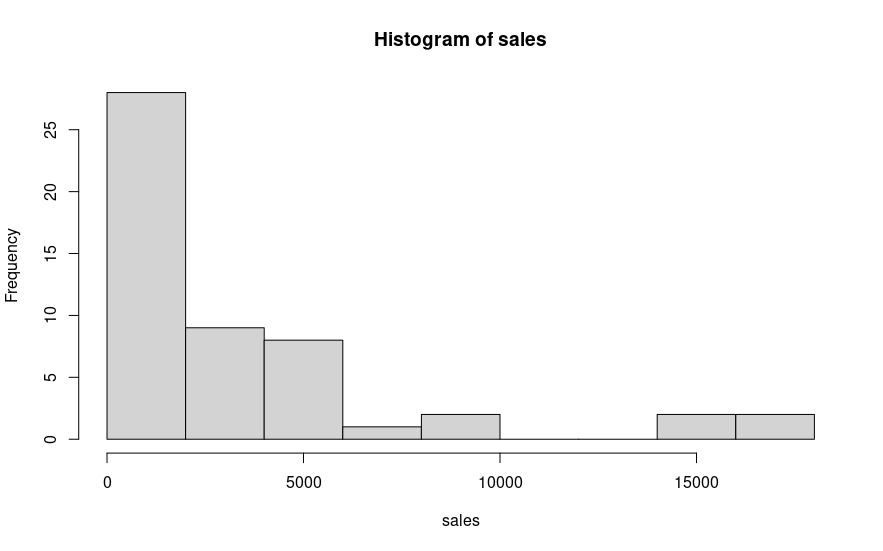
\includegraphics[width=.45\textwidth]{histSales.PNG}
  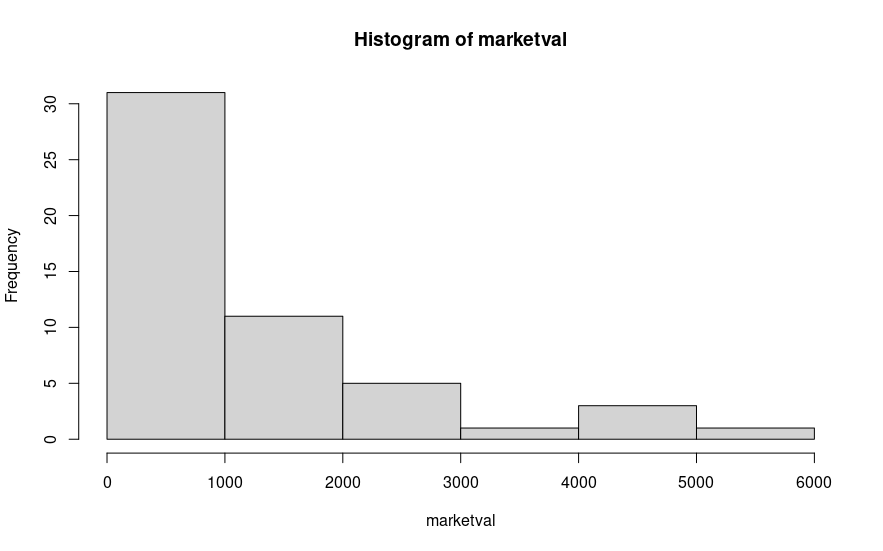
\includegraphics[width=.45\textwidth]{histMarketval.PNG}
  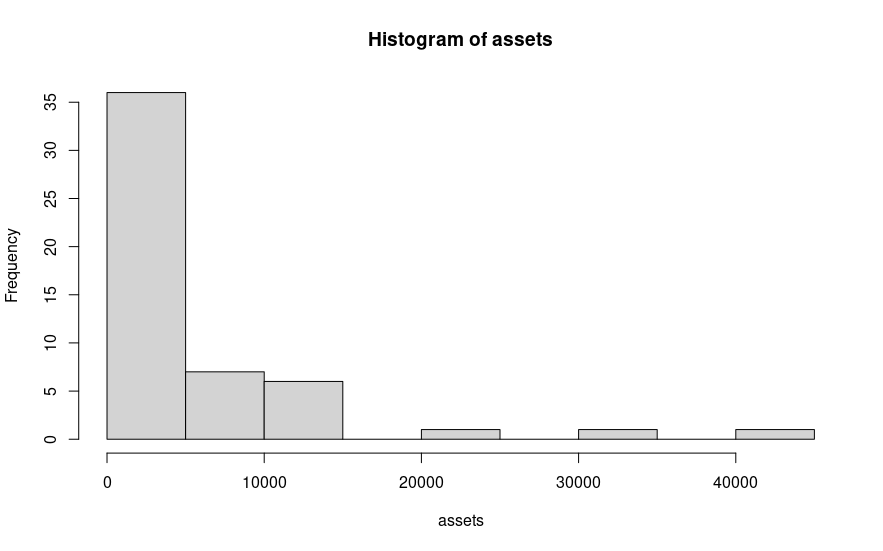
\includegraphics[width=.45\textwidth]{histAssets.PNG}
  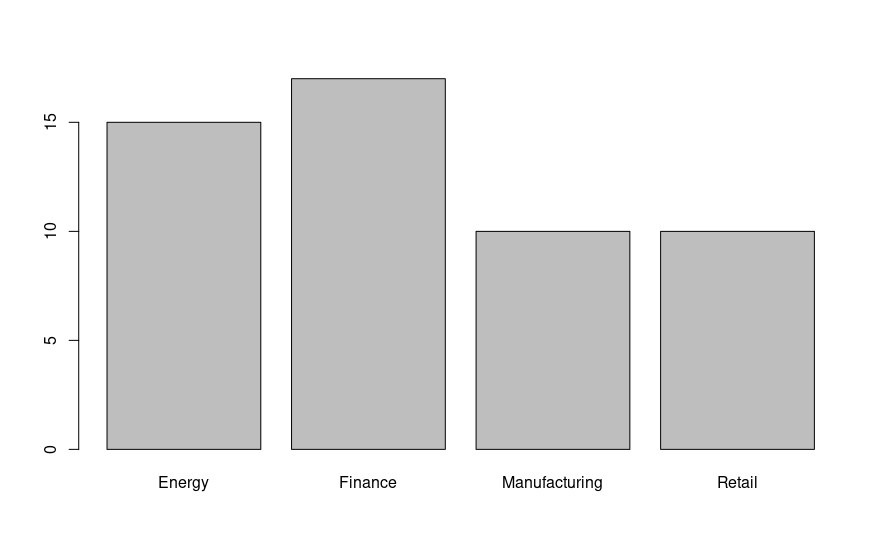
\includegraphics[width=.45\textwidth]{barSector.PNG}
  \end{center}
  \caption{De marginale verdelingen van de vier gegeven covariaten.}
  \end{figure}
  
  De bovenstaande plots geven als eerste indruk dat de financi\"ele variabelen erg scheef verdeeld zijn. Dit motiveert mogelijk een logaritmische transformatie van de financi\"ele data, waarover we hieronder nog uitgebreid zullen komen te spreken. De logtransformatie wordt echter niet evident gemaakt door de bovenstaande plots. Het is bijvoorbeeld goed mogelijk dat de correlatie tussen de continue variabelen ervoor zorgt dat de residuen van het lineaire model t\' och normaal verdeeld blijken te zijn. Dit is waarom marginale verdelingen eigenlijk te weinig informatie bieden. We zullen hier dus niet lang op blijven hangen.
  
  Over de precieze modelaannamen hebben we nog niet gesproken, zie hiervoor 1.2. Het moge echter duidelijk zijn dat dit een lineair model wordt met als verklaarde variabele \verb!sales! en als covariaten variabelen die alleen afhangen van \verb!assets!, \verb!marketval! en \verb!sector!. We verwachten in elk geval dat een groter kapitaal en een grotere marktwaarde gecorrelleerd zijn met een grotere omzet. Een bedrijf dat meer te besteden heeft zal meer investeringsmogelijkheden hebben en daardoor meer winst kunnen maken en daardoor waardevoller zijn dan een bedrijf dat minder winst maakt. 
  
  We gaan ons ori\"enteren op dit ruwe vermoeden door wat eendimensionale plots van de continue variabelen tegen elkaar, met een regressielijn ertussen. In feite zijn we hier al twee heel eenvoudige lineaire model aan het fitten, namelijk \verb!sales ~ assets! en \verb!log(sales) ~ log(marketval)! (tenzij anders aangegeven \emph{inclusief} intercept).
  
  \begin{figure}[H]
  \begin{center}
  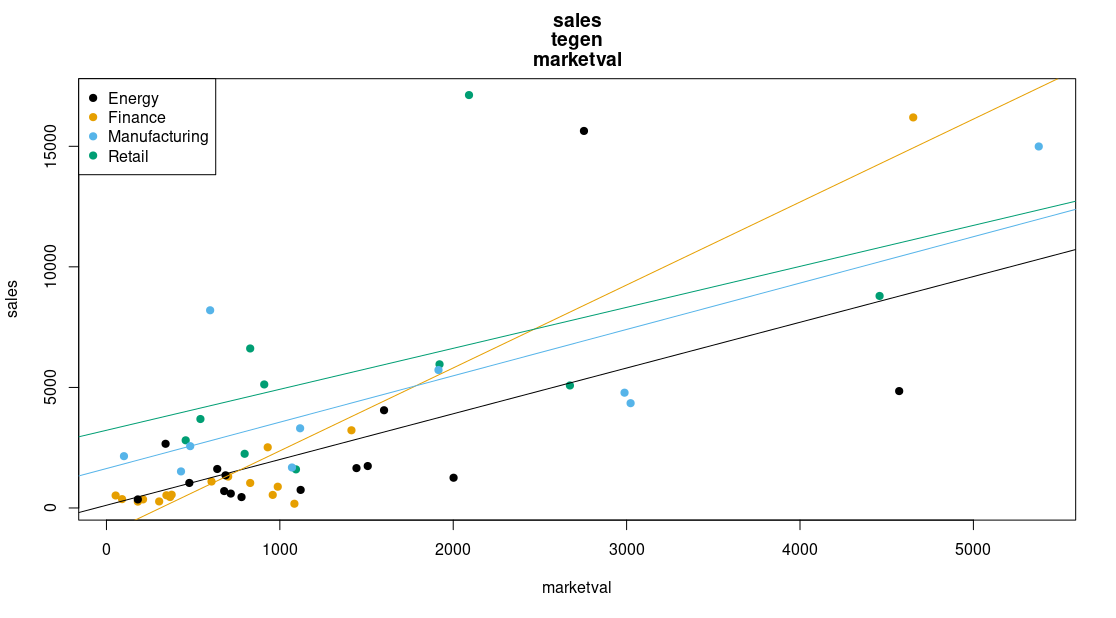
\includegraphics[scale=.25]{salesMarketval.PNG}
  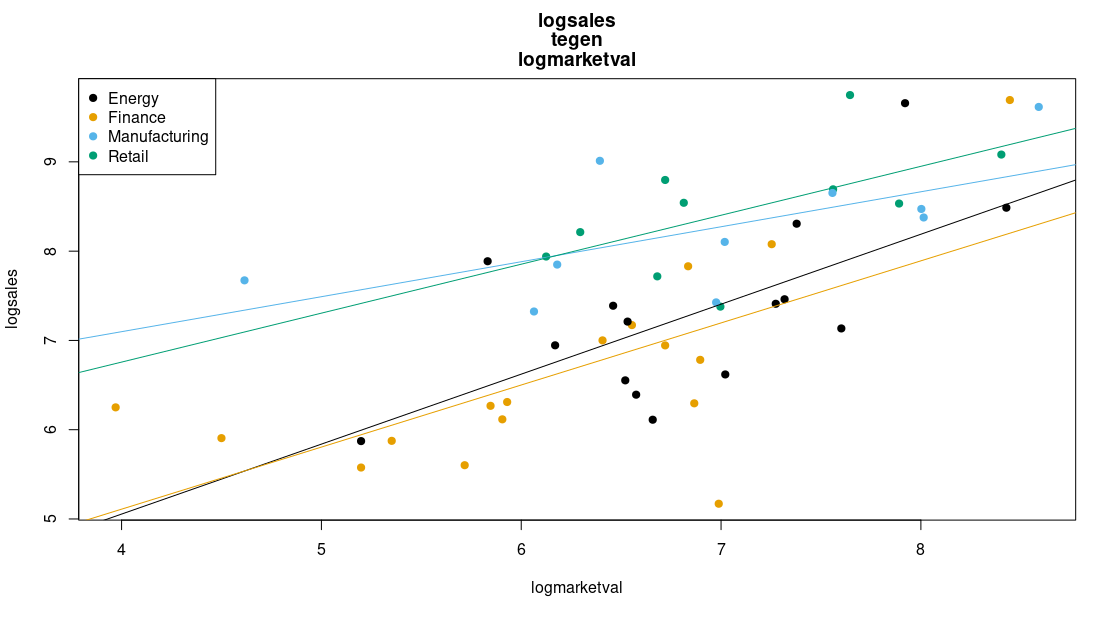
\includegraphics[scale=.25]{logsalesLogmarketval.PNG}
  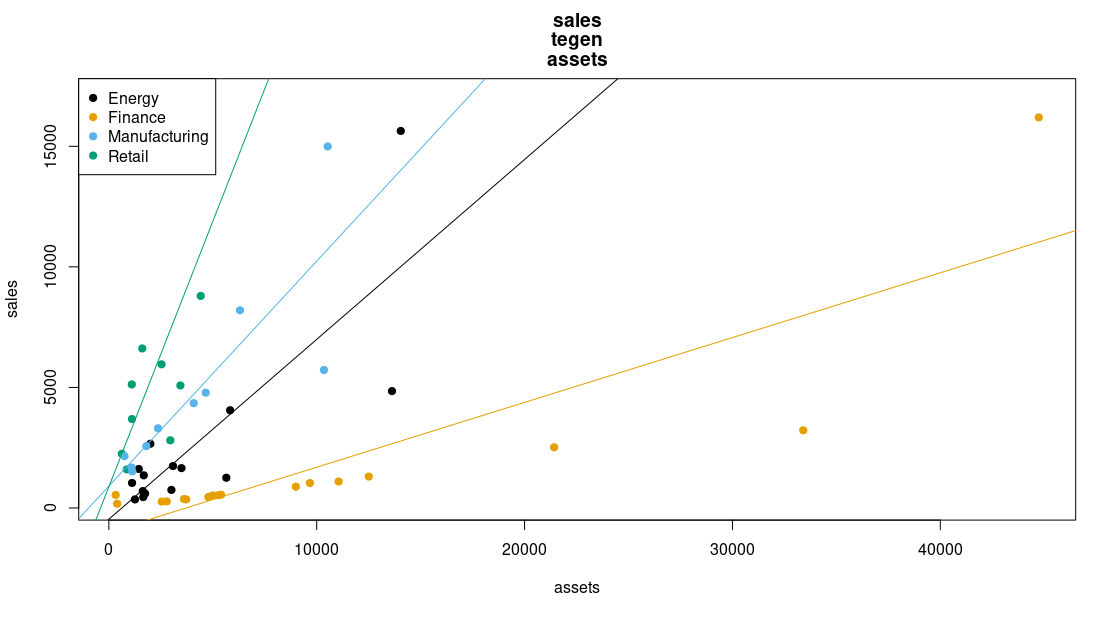
\includegraphics[scale=.25]{salesAssets.PNG}
  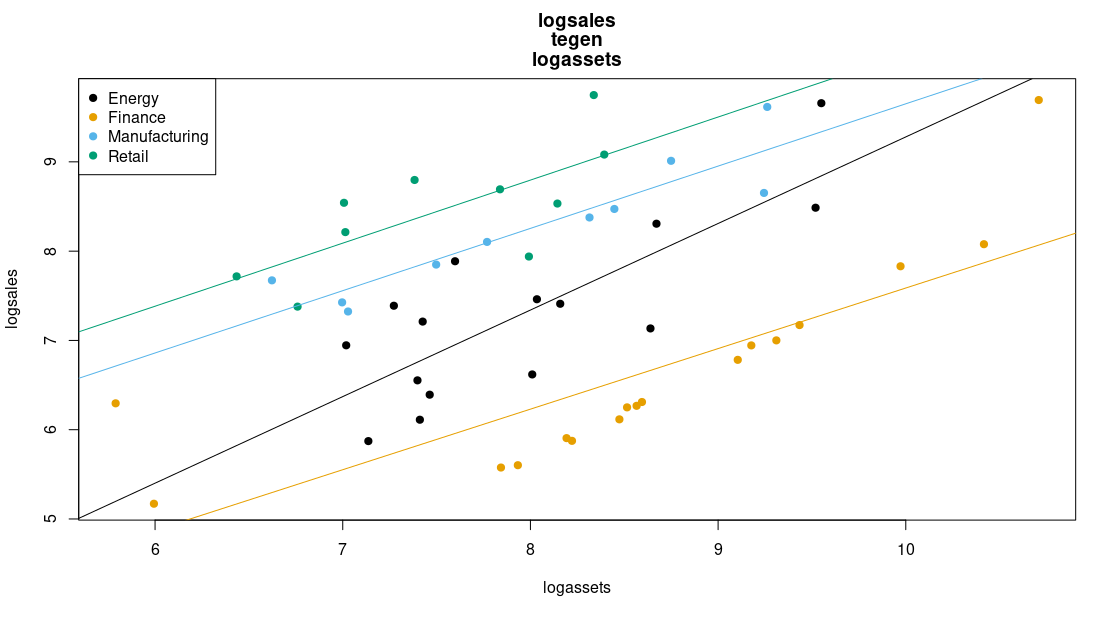
\includegraphics[scale=.25]{logsalesLogassets.PNG}
  \end{center}
  \caption{Scatterplots van sales tegen marketval, assets respectievelijk. Links zijn de `raw' datapunten genomen, rechts is een $\log$-transformatie toegepast.}
  \end{figure}
  
\subsection{Voorbehoud}
  
  Deze regressielijnen zijn in alle gevallen waarschijnlijk biased: we verklaren bepaalde variantie van $Y$ met \' e\' en covariaat terwijl er eigenlijk sprake is van verklaring door nog een andere covariaat. Dat vertekent de sterkte van de rol van de zichtbare covariaat. $Y$ komt dan mogelijk tot stand door de optelsom van de twee covariaten, maar de enkelvoudige modellen `zien' echter voor zichzelf slechts \' e\' en van de twee (relevante?) covariaten. 

  We zien in alle plots een zwakke trend, maar vooral tussen \verb!logsales! en \verb!logmarketval!. Links zien we wederom scheefheid in de data, welke duidelijk leidt tot ongewenste \emph{heteroskedasticiteit} in beide modellen: de variantie van de errors is veel groter voor grotere waarden van de covariaten.
  
\section{Model}  
\label{Model}
  We gaan een lineair model schatten met gronddata gegeven in de bovenstaande variabelen. Wanneer we over `covariaten' spreken, hebben we het over de covariaten hebben die op dat moment in dat model gekozen zijn. We doen de volgende modelaannamen voor een nog niet gekozen design-matrix $X \in \mathbb{R}^{n\times p}$ en de `stochastische' datavector $Y: \Omega \rightarrow \mathbb{R}^n$:
  
  \begin{align}
  Y = X\beta + \varepsilon \\
  \varepsilon \sim \mathcal{N}(0,\sigma^2I)
  \end{align}
  
  Later gaan we dit model uitbreiden door ons af te vragen of de varianties van de errors niet per level van \verb!sector! apart moeten worden geschat. Deze uitbreiding ziet er, formeel geformuleerd, als volgt uit:
  
  \begin{align}
  Y = \begin{pmatrix} X_{\text{m}}  \\ X_{\text{f}} \\ X_{\text{r}} \\ X_{\text{e}} \end{pmatrix}\beta + \varepsilon \\
  \varepsilon \sim \mathcal{N}(0,
  \begin{pmatrix} 
  \sigma_{\text{m}}^2I & & & \\ 
  & \sigma_{\text{f}}^2I & & \\ 
  & & \sigma_{\text{r}}^2I & \\
  & & & \sigma_{\text{e}}^2I \\
  \end{pmatrix})
  \end{align}
  
  We partitioneren de designmatrix $X$ dus in 4 blokken waar we de waarnemingen die een bepaalde sector (m, f, r, e) hebben groeperen in \' e\' en blok. Corresponderend daarmee wordt de covariantiematrix van $\varepsilon$ een diagonaalmatrix met ter hoogte van ieder blok diagonaalelementen die worden geparametriseerd door de variantie $\sigma_{\text{sector}}^2$ horend bij die sector.

\section{Onderzoeksvragen}
  In dit hoofdstuk gaan we enkele vragen formuleren bij de data die interessant kan zijn bij het analyseren van verbanden in de dataset. Aan de hand van deze vragen kunnen we verdelingsonderzoek verrichten en daarna een aantal kandidaatmodellen formuleren die ons zinvol lijken.
  
  Ik heb me bij het formuleren van de vragen gebaseerd op eigen ingeving alsook op de suggesties uit de opdracht.  
  
  De vraag is voornamelijk welk lineair model het beste $Y$ verklaart. Die vraag is niet altijd objectief. Een heel groot lineair model zal altijd meer variantie in de afhankelijke variabele opvangen omdat de kolomruimte van de designmatrix groter is dan een subset van dit model, en zal dus altijd beter presteren op de \emph{gegeven} data. De vraag is daarom ook of de opgenomen effecten wel significant bijdragen.
  
  \begin{enumerate}
  \item Is een $\log$-transformatie voor de financi\"ele variabelen zinvol?
  
  \item Is er significante variatie in conditionele verdelingen van \verb!sales! of anders \verb!logsales! afhankelijk van \verb!sector!? In woorden, is het zinvol om de effecten van de continue variabelen per sector te schatten?
  
  \item Zie in dit opzicht ook suggestie 6: is het zinvol om de \emph{variantie} in de errors per categorie te schatten? Dit is een uitbreiding op het model uit \ref{Model}. De precieze formulering is dan, of $\varepsilon \sim \mathcal{N}(0,\Sigma^2)$ met $\Sigma^2$ een diagonaalmatrix, maar nu op de diagonaal is $(\Sigma^2)_{ii} = \sigma^2_{\text{sector}}$, welke nog afhangt van de \verb!sector! van datapunt $X_{i-}$. 
  
  Dit vermoeden kunnen we toetsen met een nieuwe toetsingsstatistiek die gegeven is in de opgave. Op het eerste gezicht lijkt het zoeken naar bepaalde varianties lastiger te implementeren, maar vergeet niet dat \verb!R! gebouwd is voor dit soort vragen.
  
  Tenslotte merken we op dat de hypothese van deze toets, $H_0:\sigma_1=\sigma_2=\sigma_3=\sigma_4$ tegen $H_1: \sigma_1
  \neq \sigma_2 \neq \sigma_3 \neq \sigma_4$, steeds binnen een model geformuleerd wordt. Fitten we meerdere modellen, dan moeten we deze toets ook voor deze verschillende modellen apart uitvoeren.
  \end{enumerate}
  
\chapter{$\log$-transformatie voor financi\"ele data}
\section{Ecomische motivatie voor $\log$-transformatie}
  Er bestaat een heldere motivatie voor het $\log$-transformeren van financi\"ele data. In het geval van financi\"ele data zijn afhankelijkheden veelal ratio en niet additief. Beschouw immers de volgende (zeer eenvoudige) modellen voor de omzet van een bedrijf, afhankelijk van het kapitaal:

\begin{align}
  \text{sales} = \alpha + \beta \cdot \text{assets} \\
  \text{log(sales)} = \alpha + \beta \cdot \text{log(assets)}
\end{align}
  (N.B. deze modellen corresponderen met de twee onderste trendlijnen in figuur 1.2)
  
  Het is intu\"itief aansprekend dat wanneer het kapitaal van een bedrijf met 5\% stijgt, de marktwaarde met een evenredig (niet per se gelijk) percentage zal toenemen. Dit correspondeert met een lineaire verschuiving van $\log(\text{sales})$ (n.l. met $\log(1.05)$), en een daaruit volgende lineaire verschuiving van $\log(\text{sales})$ (n.l. met $\beta \log(1.05)$). Een uitspraak als `wanneer een retailbedrijf in kapitaal verdubbelt, zal de omzet met 50\% toenemen' correspondeert met een $\beta = \log(2)/\log(1.5)$.
  
  Wat het ongetransformeerde lineaire model postuleert, is veel minder aannemelijk. Dit verband houdt namelijk in dat per extra 1\$ in omzet de marktwaarde met $\beta$\$ zal stijgen. Maar niet voor elk kapitaalniveau zal elke extra dollar direct omgezet worden in $\beta$ extra dollar winst, om het maar even grof te formuleren. Deze toename per extra dollar noemen economen de `marginale omzet' (wij noemen het de afgeleide), en een van de centrale aannamen in de economie is juist de wet van `diminishing returns', dus dat deze marginale omzet afneemt. 
  
  Een motivatie voor deze wet is eenvoudig: bij toename van het kapitaal naar een steeds groter bedrag, zullen toch andere variabelen - zoals begrensde afzetmogelijkheden - beperkingen opleggen aan de winst. Neem bijvoorbeeld MacDonalds: dit bedrijf kan met meer kapitaal weliswaar meer restaurants openen, meer reclamezuilen huren en in nog goedkopere productiemethoden voor burgers investeren en met nog meer kwantumkorting aardappel(meel) inkopen om er frietjes van te maken, uiteindelijk is er een grens aan het aantal bezoeken per persoon per dag en dus aan de verkoop van producten. Het kan dus niet anders of de `(kapitaal $\mapsto$ winst)-functie' zal ergens beginnen te krommen naar een asymptoot.
  
  
  Het is moeilijk om deze kromming waar te nemen in de gegeven data, dus voor deze subsection zal het helaas blijven bij wat economisch gefilosofeer. De volgende motivatie voor de $\log$-transformatie is statistisch van aard en zullen we op rigoreuze wijze hard maken.
  
  Tenslotte moeten we ook de mogelijkheid overwegen om alleen de verklarende of alleen de verklaarde variabele te transformeren. Dit heeft echter geen zinvolle economische interpretatie en is daardoor moeilijk te rechtvaardigen. Bovendien worden twee verschillende eenheden met elkaar in verband gebracht: namelijk geld en ratio's van geld. Dat is ook niet erg logisch. Het komt in praktijk dan ook nooit voor.
 
\section{Statistische motivatie voor de $\log$-transformatie} 
\subsection{Heteroskedasticiteit}
  Een andere motivatie van het nemen van $\log$-transformaties heeft meer te maken met de verdeling van het logaritme van financi\"ele data. Financi\"ele data blijkt in praktijk heel scheef verdeeld te zijn. Wederom is dat logisch, want in een groot bedrijf met veel kapitaal passen veel kleine bedrijfjes met weinig kapitaal. De verhouding bedrijven met `groot kapitaal' tot bedrijven `klein kapitaal' is daardoor scheef. 
  
  Deze observatie deden we al toen we keken naar de marginale verdelingen van de financi\"ele variabelen in onze dataset (zie 1.1). We zagen de scheefheid terugkomen in de uitbijters in het scatterplot van de ongetransformeerde data.
  
  Deze uitbijters zijn desastreus voor de gepostuleerde modelaanname van \emph{homoskedasticiteit}, d.w.z. de variantie van de residuen is constant en niet gecorrelleerd met de grootte van de covariaten. Immers, als het logaritme van elke financi\"ele variabele, zeg $Z$ een vaste verdeling volgt, zoals een normale verdeling, dan volgen de financi\"ele variabelen de verdeling van $\exp(Z)$. De $\exp$-functie kromt sterk naar boven voor grotere waarden van $Z$, dus bij kleine variatie van $Z$ rond een bepaald punt $x$ is variatie van $\exp(Z)$ klein voor kleine waarden van $x$ en juist heel groot voor grote waarden van $x$. dus als $\text{log(sales)} = \alpha + \beta \cdot \text{log(assets)}$ voldoet aan homoskedasticiteit, dan $\text{sales} = \alpha + \beta \cdot \text{assets}$ z\' eker niet!
  
  We kunnen echter veel rigoureuzere uitspraken doen over deze financi\"ele variabelen met statistische toetsen. Ik wil zelfs beweren dat de marginale verdelingen van de $\log$s van de financi\"ele data inderdaad normaal zijn. Nu gaan we een Kolgomorov-Smirnov-toets uitvoeren om dit te toetsen voor de marginale verdelingen van \verb!assets!, \verb!marketval! en \verb!sales!.
  
\subsection{Kolgomorov-Smirnov-toets op normaliteit van logassets, logmarketval en logsales}  
  
  Het idee achter de KS-toets is bekend uit \emph{Inleiding in de Statistiek}. Voor $H_0: F = F_0, \ H_1: F \neq F_0$: zij $T$ de grootste absolute afwijking tussen de empirische verdelingsfunctie van de data en de nulverdeling $F_0$, dan volgt $T$ een bekende verdeling en verwerpen we voor $T$ groot genoeg.
  
  Het probleem met de KS-toets, welke ook in dat boek wordt behandeld, is dat men $F_0$ eigenlijk graag wil kiezen op basis van geschatte parameters n\' adat men de data heeft waargenomen. Wij willen nu bijvoorbeeld controleren of \verb!assets! een normale verdeling bezit, en als $F_0$ willen we graag de verdeling kiezen die als gemiddelde en variantie het waargenomen steekproefgemiddelde en de waargenome variantie van \verb!assets! bezit. Dit mag niet, omdat $F_0$ een vaste verdeling moet zijn die niet mag afhangen van de data dus ook niet van de schatters $\bar{X_n}$ en $S^2_X$.
  
  Een uitbreiding van de KS-statistiek $T^*$ (zie wederom \emph{Inleiding in de Statistiek}) is gegeven voor het tupel van hypothesen $H_0: F \in \mathcal{F}_0, \ H_1: F \not \in \mathcal{F}_0$. Hierbij is $\mathcal{F}_0$ een familie van verdelingsfuncties (bijvoorbeeld een locatieschaalfamilie), je zou kunnen zeggen een model. $T^*$ is nu de grootste absolute deviatie tussen de empirische verdelingsfunctie en de verdelingsfunctie die geparametriseerd is door de maximum-likelihoodschatters van de parameters. In praktijk zijn deze voor een normale verdeling $\overline{X_n}$ en $S_X$ en geeft dit de volgende toetsingsgrootheid:

  \begin{equation}
    T^* = \sup_{x\in \mathbb{R}} | \mathbb{F}_n(x) - \Phi(\frac{x-\overline{X_n}}{S_X})|
  \end{equation}  	
	
   We zijn nu ge\"interesseerd in de verdeling van $T^*$ onder de nulhypothese, zodat we bij zeer incompatibele waarden van $T^*$ de nulhypothese kunnen verwerpen en een $p$-waarde kunnen geven. Merk echter op dat de verdeling van $T^*$ in zijn geheel niet triviaal is. We zouden deze kunnen simuleren, maar ook dan is de vraag met welk element (welke normale verdeling dus) van $\mathcal{F}_0$ we dit zouden moeten doen. Immers hangt de verdeling van $T^*$ misschien wel af van de ware parameter van de normale verdeling? 
   
   Op p.146 van \emph{Inleiding in de Statistiek} staat gelukkig dat de verdeling van $T^*$ hetzelfde is onder ieder element van $\mathcal{N}$. We nemen dus een standaardnormale verdeling en bepalen met behulp van simulatie de nulverdeling van $T^*$: we nemen een simulatiesteekproef van 1,000,000.

  Vervolgens bepalen we de KS-test statistiek met de ingebouwde functie in \verb!R!. Dit doen we voor \verb!assets!, \verb!marketval! en \verb!sales!, en dus ook voor \verb!logassets!, \verb!logmarketval! en \verb!logsales!. Dit zijn, zoals de namen al zeggen, de $\log$-getransformeerde variabelen.
  
  Kortheidshalve is de \verb!R!-code uit de tekst gelaten.
  
  \begin{figure}[H]
  \begin{center}
  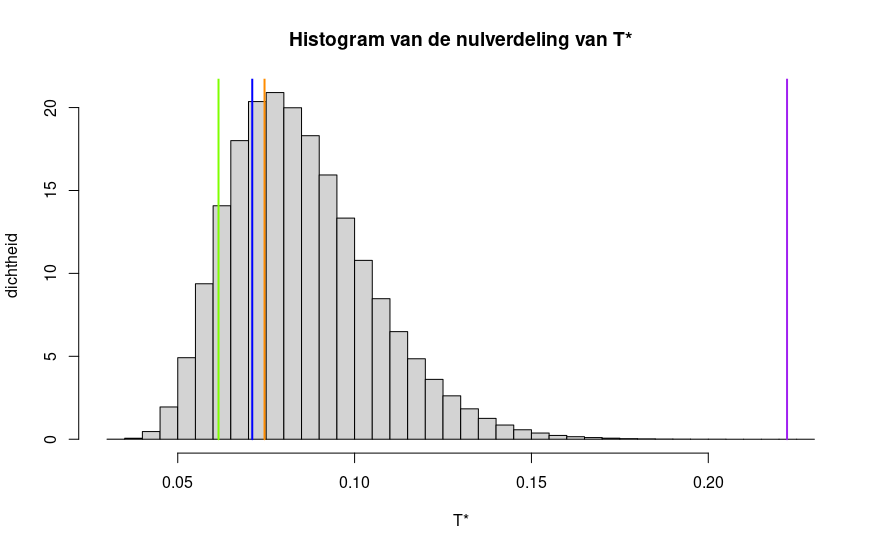
\includegraphics[scale=.5]{KSTestLog.PNG}
  \begin{multicols}{2}
  \begin{verbatim}
 > pvalue(Tlogsales)
[1] 0.663722
> pvalue(Tlogassets)
[1] 0.897291
> pvalue(Tlogmarketval)
[1] 0.734819

> pvalue(Tsales)
[1] 1e-06
> pvalue(Tassets)
[1] 0
> pvalue(Tmarketval)
[1] 0
  \end{verbatim}
  \end{multicols}
  \end{center}
  \caption{De gesimuleerde nulverdeling van $T^*$. In de grafiek zijn ook de werkelijke waarden van $T^*$ gegeven voor de dataset: groen: logassets, blauw: logmarketval, oranje: logsales, paars, rood, magenta: overlappen elkaar, dit zijn de ongetransformeerde variabelen. We zien dat deze zeer incompatibel met $H_0$ zijn. Onderstaand de $p$-waarden bij de toets.}
  \end{figure}   
  
  We kunnen met grote zekerheid zeggen dat de `raw' data niet normaal verdeeld is: de $p$-waardes zijn heel klein. Daarentegen is het best aannemelijk (niet verwerpbaar) dat de getransformeerde data wel normaal verdeeld is. Merk overigens op dat dit niet hoeft te betekenen dat de residuen van $Y$ na enige fit dat ook zijn. Toch bleek uit de plots onder \ref{Verdelingsonderzoek} dat voor de raw data zichtbare heterogeneiteit te zien was. Om deze, en de hierbovenstaande theoretische motivatie is besloten de regressiemodellen alle te fitten voor de $\log$ van de financi\"ele data.
  
\chapter{Een Na\"ief Model en Uitbreidingen}

  Dit hoofdstuk geeft een overzicht van de (nu nog homoskedastische) modellen die geformuleerd worden in dit werkstuk. We geven eerst het meest eenvoudige model. Daarna breiden we dit model uit door interactietermen toe te voegen.
  
  Pas in het volgende hoofdstuk zullen we ingaan op een vergelijking van de modellen. Dan ook pas zullen we een theoretisch kader ontwikkelen voor de implicaties van het wel/niet opnemen van variabelen als regressors, en relevante toetsen bespreken (zoals de $F$-toets).
  
\section{Basale Model}
\label{Basale Model}
  Dit model heeft 6 parameters, namelijk een intercept, twee voor de regressors \verb!logassets! en \verb!logmarketval! en nog drie voor de dummy's die corresponderen met de overige sectoren. Als basislevel van \verb!sector! wordt ``Energy'' genomen, dat doet \verb!R! zelf (alfabetische volgorde van de levels) (en welk level het baselevel wordt is niet zo relevant, zolang we dit maar voor elk ander model consistent hetzelfde kiezen, anders wordt het moeilijker de modellen te vergelijken). De summary ziet er als volgt uit:
  
  \begin{figure}[H]
  \begin{verbatim}
lm(formula = logsales ~ logmarketval + logassets + sector)

Residuals:
    Min      1Q  Median      3Q     Max 
-0.8064 -0.3430 -0.1136  0.2910  1.1818 

Coefficients:
                    Estimate Std. Error t value Pr(>|t|)    
(Intercept)          0.67694    0.66809   1.013 0.316244    
logmarketval         0.27718    0.09436   2.937 0.005157 ** 
logassets            0.59310    0.09065   6.543 4.43e-08 ***
sectorFinance       -0.85830    0.21671  -3.961 0.000258 ***
sectorManufacturing  0.90871    0.21757   4.177 0.000130 ***
sectorRetail         1.34954    0.22439   6.014 2.76e-07 ***
---
Signif. codes:  0 ‘***’ 0.001 ‘**’ 0.01 ‘*’ 0.05 ‘.’ 0.1 ‘ ’ 1

Residual standard error: 0.5327 on 46 degrees of freedom
Multiple R-squared:  0.8151,	Adjusted R-squared:  0.795 
F-statistic: 40.56 on 5 and 46 DF,  p-value: 9.248e-16
  \end{verbatim}
  \caption{De summary van de fit. De geschatte co\"effici\"enten staan in de kolom `Estimate'. }
  \end{figure}  

\chapter{Theorie over Lineaire modellen en Modelselectie}

  Uitgaande van het model uit \ref{Model} is er veel statistische theorie rondom het schatten en uitvoeren van toetsen op deze modellen. Wij benoemen hier enige relevante theorie die helpt bij het interpreteren van de summary's uit het voorgaande hoofdstuk. Ook vormen we wat nieuwe theorie voor de vraag, hoe te toetsen of een regressor aan het model kan worden toegevoegd of moet worden weggelaten.

\section{Schatten}
  \verb!R! schat lineaire modellen door de schatter $\hat{\beta}$ zodanig te kiezen dat de kwadratensom van de residuen, $\norm{Y-X\hat{\beta}}^2$, geminimaliseerd wordt. Dit heet de kleinste-kwadratenschatter. Onder de aanname van normaal verdeelde errors/residuen met een constante variantie (homoskedasticiteit) is deze schatter equivalent met de maximum-likelihood schatter.
  
  Deze schatter heeft een directe formule, welke gelijk is aan de berekening van de vector $\hat{beta}$ die een lineaire combinatie $X\hat{\beta}$ maakt die precies de loodrechte projectie van $Y$ op $V$, de colspace van $X$, is.
  
  Een afleiding van de formule is te vinden in \emph{Inleiding in de Statistiek}. Hier staat hij:
  
  \begin{equation}
  \label{kleinste kwadraten schatter}
  \hat{\beta} = (X^tX)^{-1}X^tY
  \end{equation}
  
  Deze schatter is zuiver onder de modelaannames.

\section{Restricted Models}

  Het lastige van modellen fitten, is dat schattingen voor parameters in een model niet goed met de werkelijke parameterwaarden overeen zullen komen, wanneer een gepostuleerd model niet overeenkomt met het werkelijke `model'. Bij lineaire modellen ligt dit `overeenkomen met het werkelijke model' vaak in de keuze om een bepaalde variabele wel of niet op te nemen in het model.
  
  Stel dat het `werkelijke model' van de volgende vorm is:
  
  \begin{align}
  Y = X_0\beta_0 + X_1\beta_1 + \varepsilon \\
  \varepsilon \sim \mathcal{N}(0,\sigma^2I)
  \end{align}
  
  In andere woorden, deel in \ref{Model} de designmatrix op in $X = \begin{pmatrix} X_0 & X_1 \end{pmatrix}$ en de parameter in ${\beta = \begin{pmatrix} \beta_0 \\ \beta_1 \end{pmatrix}}$. 
  
  We kunnen het `wel of niet ertoe doen' en het `wel of niet opnemen in het model' van variabelen uit $X$ nu als volgt formuleren:
  
  \begin{enumerate}
  \item \label{restricted} Als we $X_1$ niet opnemen in het model, maar deze w\' el relevant is, dan schatten we een zogeheten `restricted model'. De aanname van het model is dus $\beta_1 = 0$. Noem de schatter van $\beta_1$ onder deze aanname $\hat{\beta}_R$.
  
  \item \label{te uitgebreid} Als we $X_1$ wel opnemen in het model, maar in werkelijkheid is deze niet relevant, i.e. $\beta_1 = 0$ in het werkelijke model, dan schatten we $\beta_0$ en $\beta_1$ dus beide terwijl we eigenlijk alleen $\beta_0$ hoeven te schatten, en wel op basis van alleen $X_0$.
  \end{enumerate}
  
  Intu\"itief is duidelijk dat \ref{restricted} leidt tot een onzuivere schatting van $\beta_0$, doordat we mogelijk een effect van $X_1$ onterecht toeschrijven aan $X_0$. Evenzo is duidelijk dat in \ref{te uitgebreid}, als $X_1$ geen effect heeft in het werkelijke model, we ook naar verwachting $\hat{\beta}_1$ als 0 zullen schatten en $\hat{\beta}_0$ als $\beta_0$, dus dat de schatters wel zuiver zullen blijven. Maar ook is duidelijk dat we extra variantie introduceren in het schattingsproces, doordat we nu rekening moeten houden met de extra toegevoegde random regressors $X_1$.
  
  We zullen deze intu\"itie nu wiskundig hard maken, door de schatters $\hat{\beta}_R$ uit \ref{restricted} en $\hat{\beta}_0$ uit \ref{te uitgebreid} uit te drukken in de ware parameters:
  
\subsection{Onterecht Restricted}

  \begin{align*}
  \hat{\beta}_R &= (X_0^tX_0)^{-1}X_0^tY \\ 
  &= (X_0^tX_0)^{-1}X_0^t(X_0\beta_0 + X_1\beta_1 + \varepsilon) \\
  &= \beta_0 + (X_0^tX_0)^{-1}X_0^tX_1\beta_1 + (X_0^tX_0)^{-1}X_0^t\varepsilon
  \end{align*}
  
  We zien dat deze schatter een verwachte waarde heeft van $\beta_0 + (X_0^tX_0)^{-1}X_0^tX_1\beta_1$. Er is dus een onzuiverheid $(X_0^tX_0)^{-1}X_0^tX_1\beta_1$, welke groter wordt naarmate $\beta_1$ verder afwijkt van $0$. Dat is intu\"itief ook logisch, want het restricted model doet onterecht de aanname dat $\beta_1=0$; hoe fouter deze aanname, hoe fouter onze schatter wordt.
  
  Men kan echter ook aantonen
  
\subsection{Onterecht te Uitgebreid}
  Schrijf eerst de afbeelding $\beta \mapsto \beta_0: \mathbb{R}^{p_0+p_1} \rightarrow \mathbb{R}^{p_0}$ als matrix $K = \begin{pmatrix} I_{p_0} & 0 \end{pmatrix}$. 
  \begin{align*}
  \hat{\beta}_0 &= K\hat{\beta} = K(X^tX)^{-1}X^tY \\ 
  &= K(X^tX)^{-1}X^t(X_0\beta_0 + \varepsilon) \\
  &= K(X^tX)^{-1}X^t(X\begin{pmatrix} \beta_0 \\ 0 \end{pmatrix} + \varepsilon) \\
  &= K \begin{pmatrix} \beta_0 \\ 0 \end{pmatrix} + K(X^tX)^{-1}X^t\varepsilon \\
  &= \beta_0 + K(X^tX)^{-1}X^t\varepsilon 
  \end{align*}
  
  De verwachting hiervan is precies $\beta_0$, dus de schatter is zuiver.
  Men kan met wat extra werk laten zien dat $(X_0^tX_0)^{-1}X_0^t$ 

\section{Toetsen voor modeluitbreidingen en -restricties}

  We willen nu toetsen of een model, dat (in regressores) een subset van een ander model is, significant slechter verklaard dan het grotere model. In andere woorden, we toetsen of de parameters in het verschil van de modellen gelijk aan nul kunnen worden gekozen. De hypothesen zien eruit als:
  
\chapter{Vergelijking van de Modellen}

\

  
\end{document}
